\documentclass[10pt,utf8]{beamer}

\mode<presentation> {
%  \usetheme{Boadilla}
  \usetheme{Madrid}
%	\usetheme{Fzu}
  \setbeamercovered{transparent}
}

\usepackage{palatino}
\usepackage{graphicx}
\usepackage{array}
\usepackage{color}
\usepackage{subfigure}
\usepackage{colortbl}
\usepackage{amsmath}
\usepackage{hyperref}
\usepackage{listings}
\usepackage{fancyvrb}

\setbeamertemplate{caption}{\raggedright\insertcaption\par} %turn off caption prefix ("Figure")

\title{OpenJDK project Loom}
\author{Vojtech Juranek}
\institute[Red Hat]{oVirt storage team}
\date{2.~3.~2021}

\lstdefinestyle{java}{
	basicstyle          = \large\ttfamily,
	language            = java,
	numbers             = left,
	numberstyle         = \small,
	stepnumber          = 1,
	numbersep           = 5pt,
	backgroundcolor     = \color{white},
	showspaces          = false,
	showstringspaces    = false,
	showtabs            = false,
	frame               = single,
	tabsize             = 2,
	captionpos          = b,
	breaklines          = true,
	breakatwhitespace   = false,
	morestring          = [b]",
	stringstyle         = \color{blue},
	keywordstyle        = \color{magenta},
	commentstyle        = \color{gray},
	identifierstyle     = \color{black},
	moredelim           = **[is][\bfseries]{`}{`},
	moredelim           = **[is][\color{magenta}]{$}{$}, 
	fancyvrb            = true,
}


\begin{document}

\begin{frame}
	\titlepage
\end{frame}

\begin{frame}[fragile]
    \frametitle{Java concurrency}
    Low-level thread: \texttt{java.lang.Threads} class and \texttt{java.lang.Runnable}.
    \begin{lstlisting}[style=java]
Runnable task = new MyRunnable();
Thread thread = new Thread(task);
thread.start();
    \end{lstlisting}
\end{frame}

\begin{frame}[fragile]
    \frametitle{Java concurrency}
    High-level Executor framework:
    \begin{lstlisting}[style=java]
Runnable task = new MyRunnable();
ExecutorService executor = Executors.newFixedThreadPool(NUM_THREADS);
executor.execute(task);
    \end{lstlisting}
    
    \vspace{0.5cm}
    \begin{lstlisting}[style=java]
Runnable task = new MyRunnable();
ExecutorService executor = Executors.newFixedThreadPool(NUM_THREADS);
Future<?> f = executor.submit(task);
    \end{lstlisting}
\end{frame}

\begin{frame}
    \frametitle{Java threads}
    \begin{itemize}
        \item 1:1 mapping to OS threads.
        \item Memory heavy (MBs).
        \item Context switching is time consuming.
        \item Creation is expensive.
    \end{itemize}
\end{frame}

\begin{frame}
    \frametitle{Thread pooling}
    \begin{itemize}
        \item Doesn't solve memory overhead and context switching, just creating overhead.
        \item Issues with \texttt{ThreadLocal} and thread interrupts.
    \end{itemize}
\end{frame}

\begin{frame}
    \frametitle{Asynchronous programming}
    \begin{itemize}
        \item Breaking tasks into smaller ones.
        \item Better CPU utilization, as blocking tasks (typically IO) are waiting in a queue instead blocking thread.
        \item Chaining usually via callbacks.
    \end{itemize}
\end{frame}

\begin{frame}[fragile]
    \frametitle{Java concurrency}
    Async. constructs added in Java 8 (e.g. CompletableFuture):
    \begin{lstlisting}[style=java]
public String myFunction(int a) {...}
CompletableFuture<String> cf = CompletableFuture.supplyAsync(() -> myFunction(10));
cf.thenAccept(result -> System.out.println(result));
    \end{lstlisting}
And many other ways how to run function asynchronously, e.g.:
    \begin{lstlisting}[style=java]
public String myFunction(int a) {...}
Stream.of(1, 2).parallel().forEach(i -> myFunction(i));
    \end{lstlisting}
\end{frame}

\begin{frame}[fragile]
    \frametitle{Asynchronous frameworks}
    \begin{itemize}
        \item \href{https://vertx.io/}{\textcolor{blue}{vert.x}}
        \item \href{https://netty.io/}{\textcolor{blue}{Netty}\textcolor{black}}
        \item ...
    \end{itemize}

    \vspace{0.5cm}

Vert.x example:
    \begin{lstlisting}[style=java]
vertx.createHttpServer().requestHandler(r -> {
  r.response()
    .putHeader("content-type", "text/plain")
    .end("Hello from Vert.x!");
}).listen(8080);
    \end{lstlisting}
\end{frame}

\begin{frame}[fragile]
    \frametitle{Handling error in async. code}
Netty example:
    \begin{lstlisting}[style=java]
ChannelFuture f = ctx.writeAndFlush(b);
f.addListener(writeFailed);

$private$ $final$ ChannelFutureListener writeFailed = (ChannelFuture future) -> {
    if (!future.isSuccess()) {
        future.cause().printStackTrace();
        future.channel().close();
    }
};
    \end{lstlisting}
\end{frame}

\begin{frame}
  \frametitle{Synchronous vs. asynchronous}
  \begin{columns}
        \column{0.6\textwidth}
            Synchronous:
            \begin{itemize}
                \item Simple to reason about it.
                \item Blocking.
                \item Less scalable.
            \end{itemize}
            
            \vspace{0.5cm}
            
            Asynchronous:
            \begin{itemize}
                \item Better scales.
                \item Harder to reason about it.
                \item ``Callback hell''.
                \item To get maximum benefit from it, all parts have to be asynchronous.
                \item Can be problematic to make it working with legacy synchronous code.
            \end{itemize}
            
        \column{0.4\textwidth}
            \begin{figure}
                \centering
                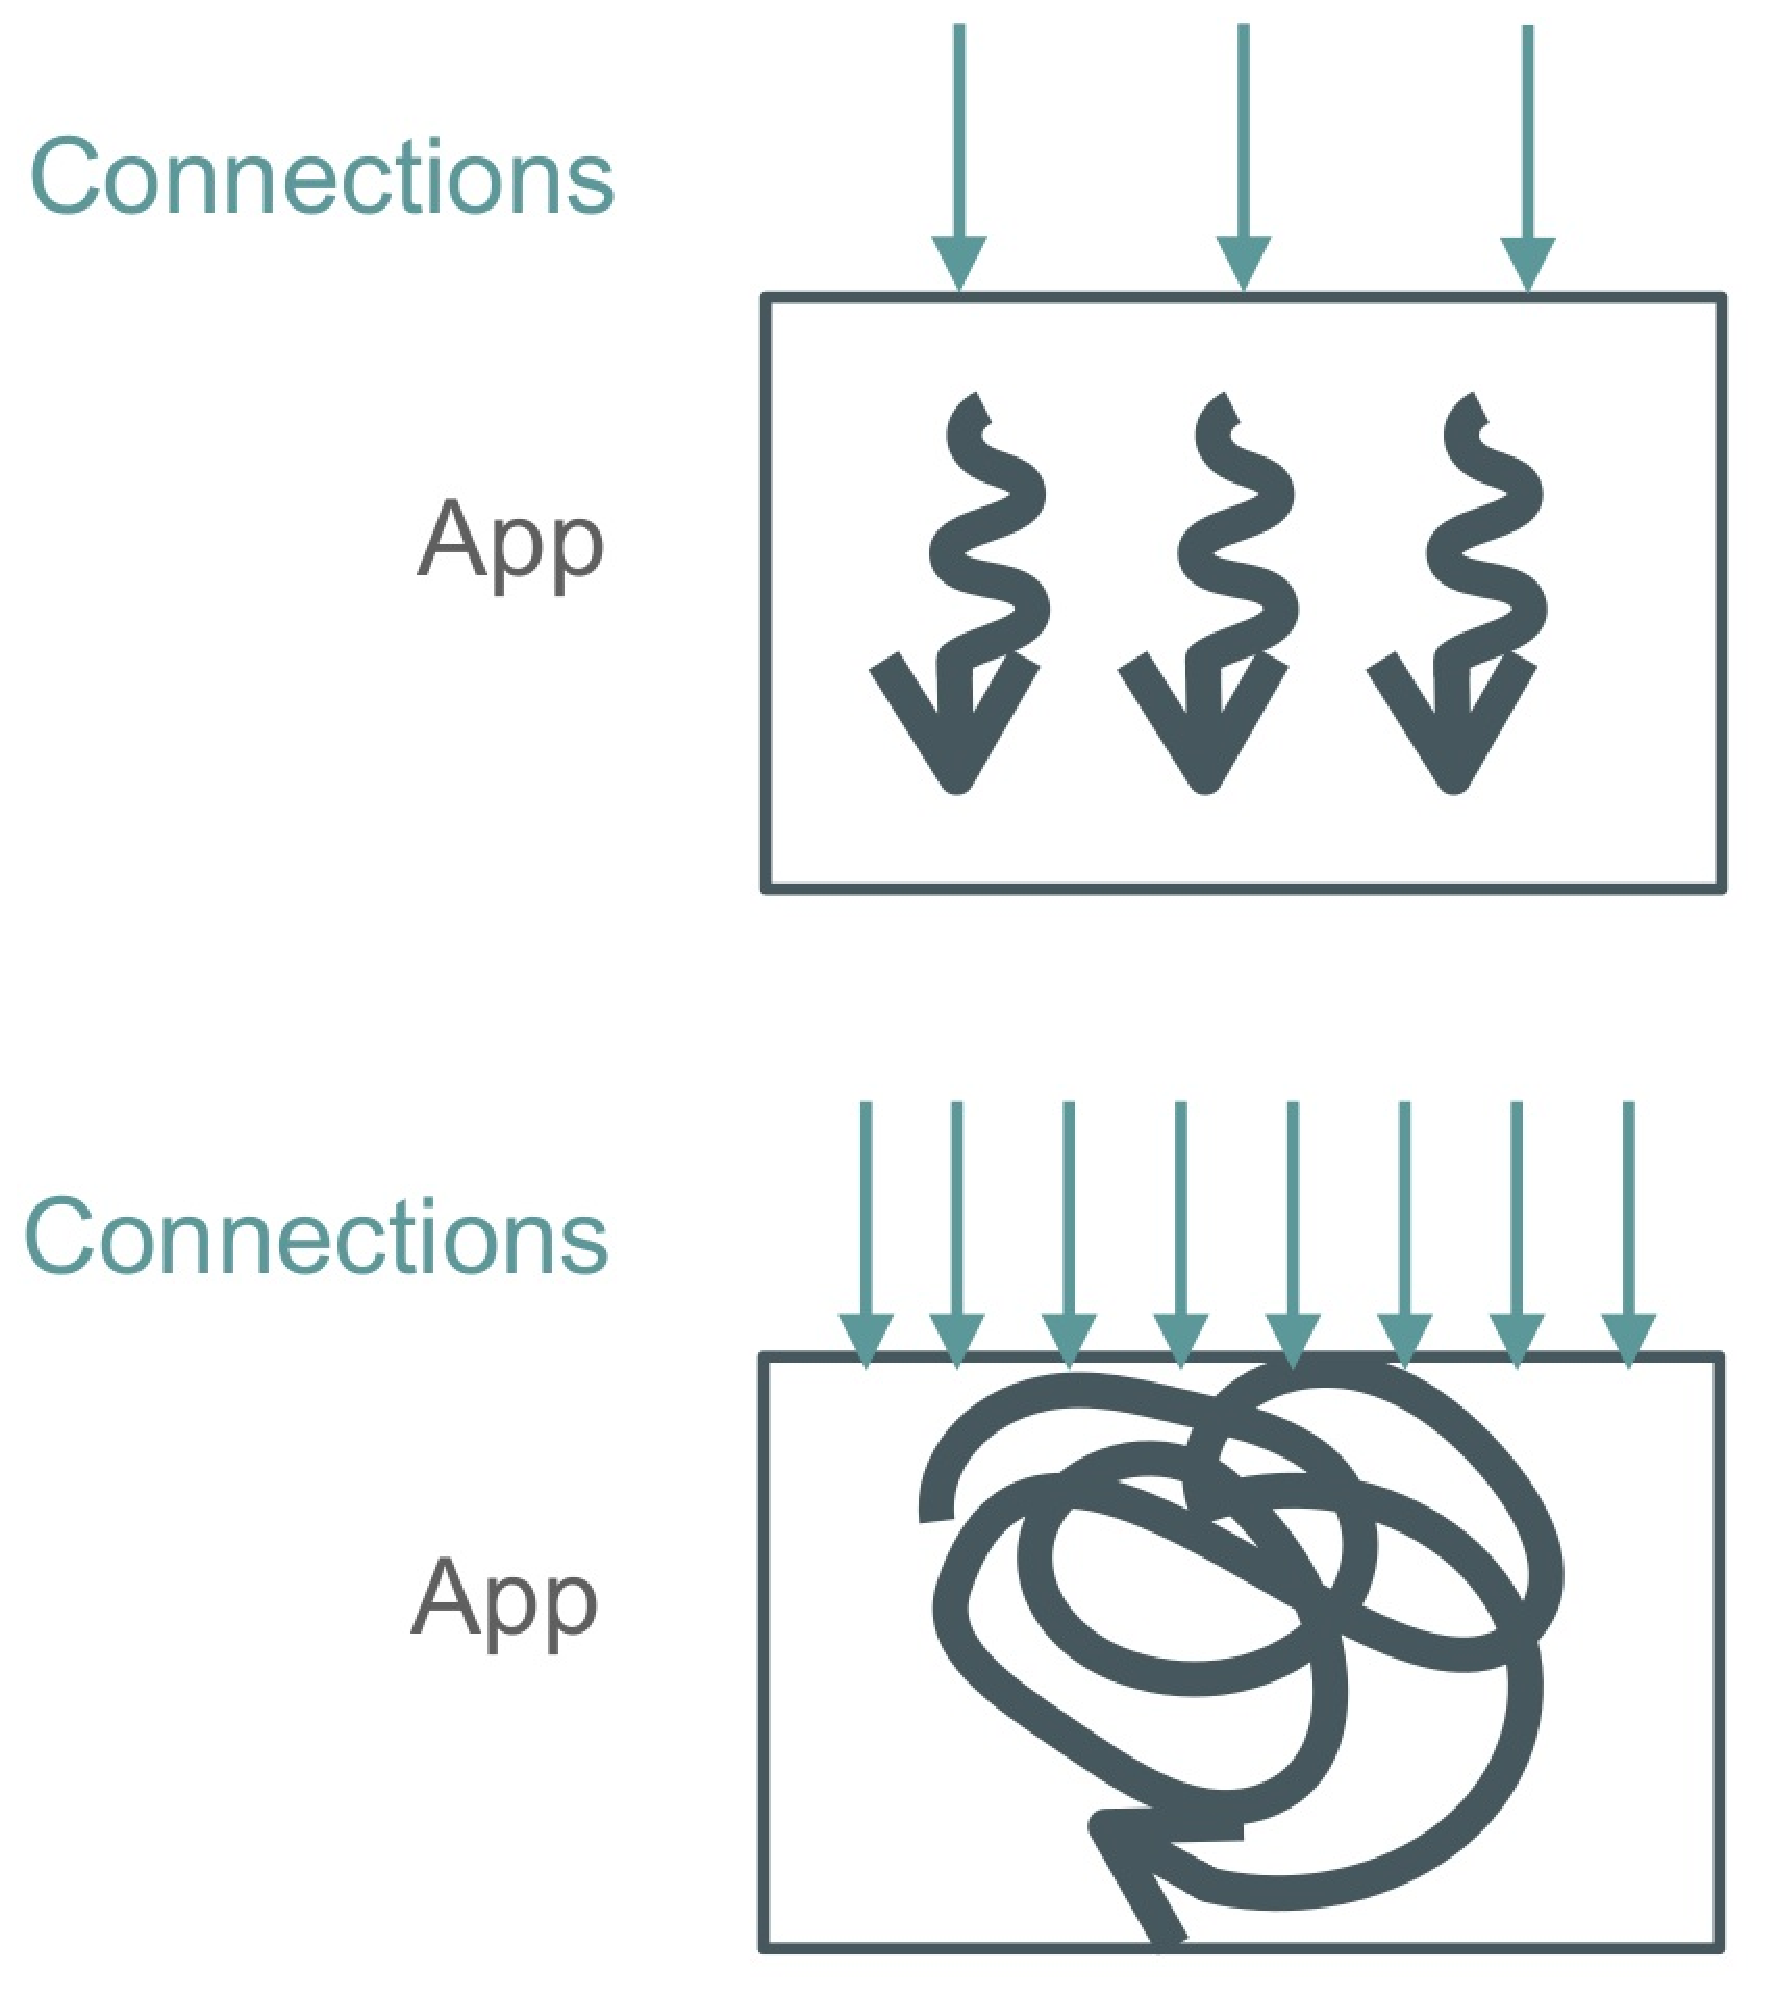
\includegraphics[height=5cm]{./img/sync_vs_async.eps}
                \caption{\tiny{Source: \url{http://cr.openjdk.java.net/~alanb/loom/Devoxx2018.pdf}}}
            \end{figure}
    \end{columns}
\end{frame}

\begin{frame}
    \frametitle{Java threads}
    What about having positives from both approaches:
    \begin{itemize}
        \item Code like synchronous code.
        \item Work like asynchronous code.
    \end{itemize}
    
    \begin{figure}
        \centering
        
\includegraphics[height=3cm]{./img/virt_threads.eps}
        \caption{\tiny{Source: \url{http://cr.openjdk.java.net/~alanb/loom/Devoxx2018.pdf}}}
    \end{figure}
\end{frame}

\begin{frame}
  \frametitle{Project Loom}
	\begin{itemize}
		\item \url{https://wiki.openjdk.java.net/display/loom/Main}
		\item Virtual threads
		\item Structured concurrency
	\end{itemize}
\end{frame}

\begin{frame}
    \frametitle{Virtual threads}
    \begin{figure}
        \centering
        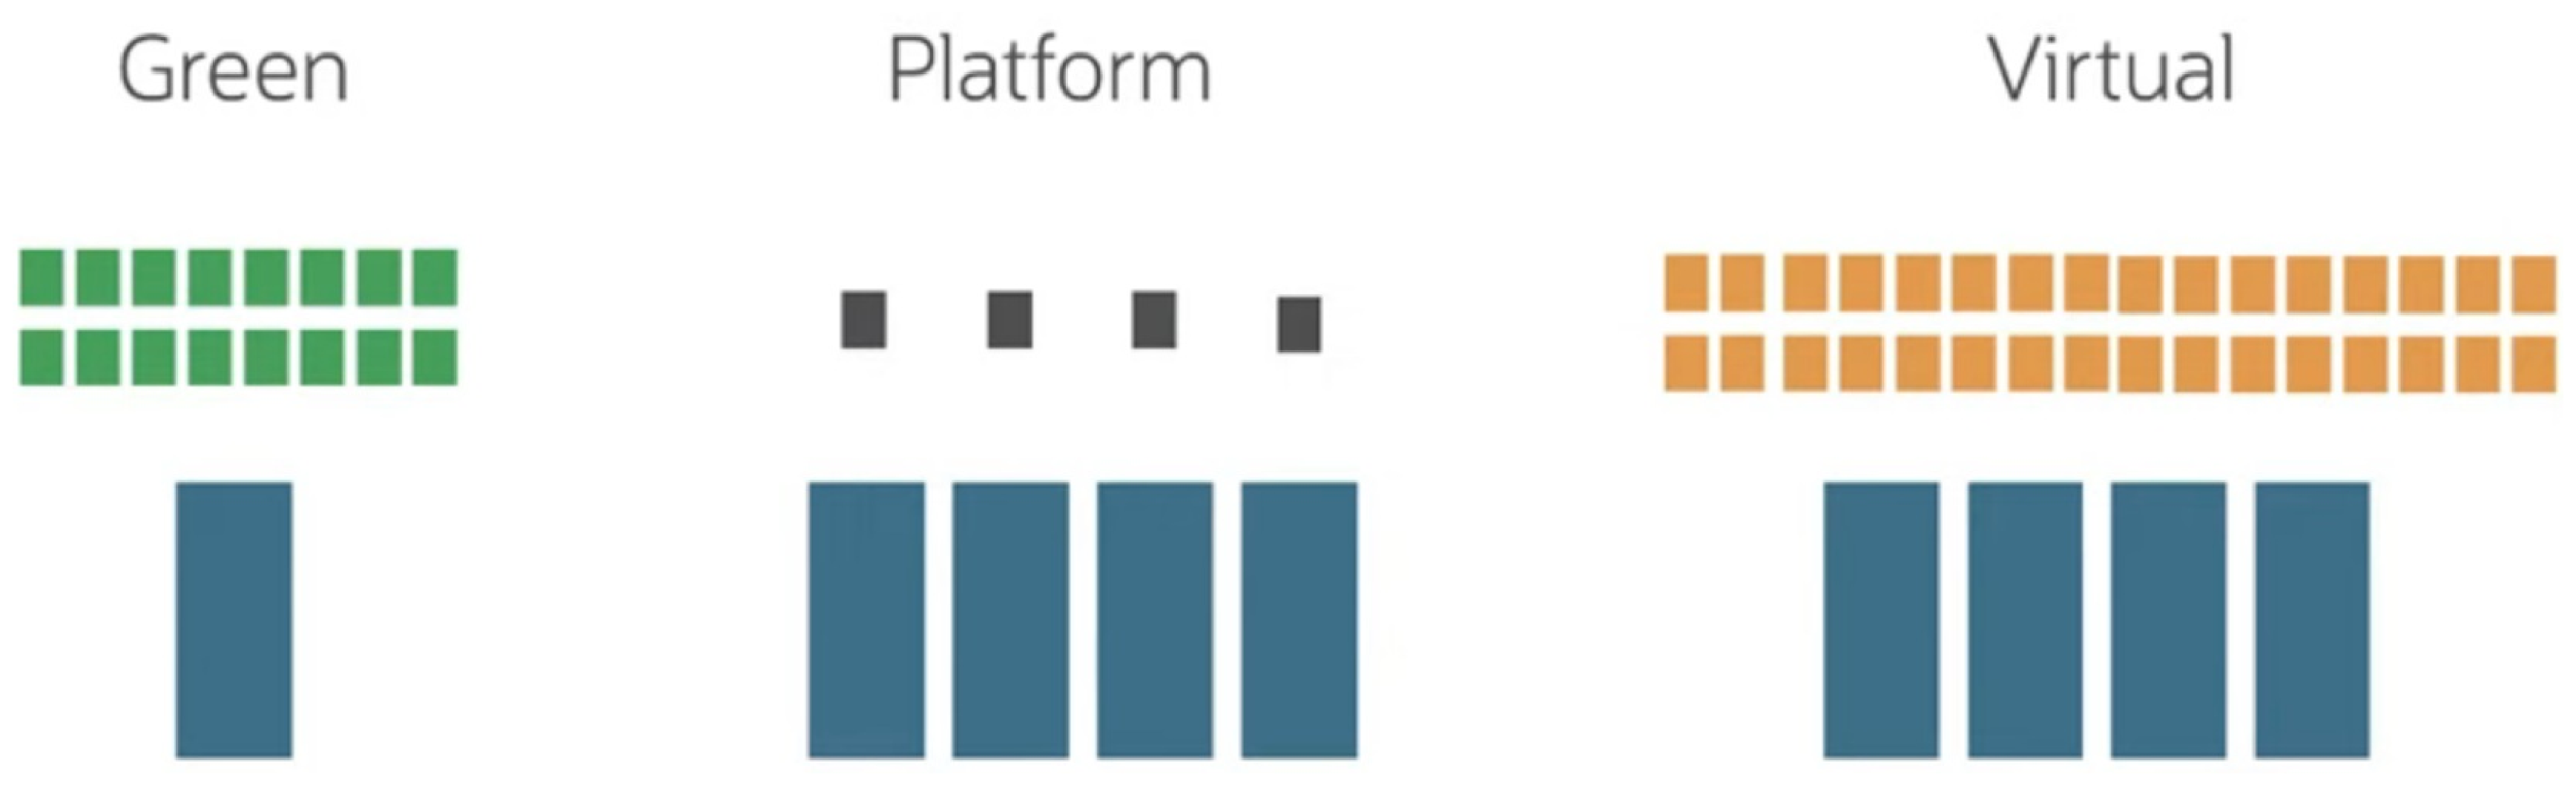
\includegraphics[height=3cm]{./img/thread_history.eps}
        \caption{\tiny{Source: \url{https://2020.accento.dev/talks/project-loom/}}}
    \end{figure}
\end{frame}

\begin{frame}[fragile]
	\frametitle{Virtual threads}
        \begin{itemize}
            \item Not bound to kernel thread (blocking in virtual thread doesn't block kernel thread).
            \item Cheap to create.
            \item Very low memory overhead.
            \item Future compatible (older code can benefit from new features).
        \end{itemize}

        \vspace{1cm}
        
	\begin{lstlisting}[style=java]
var thread = Thread.startVirtualThread(() -> System.out.println("Virtual thread!"));
thread.join();
	\end{lstlisting}
\end{frame}

\begin{frame}[fragile]
    \frametitle{Virtual threads}
    
    \begin{lstlisting}[style=java]
Thread thread = Thread.startVirtualThread(runnable);
    \end{lstlisting}
    
    \begin{lstlisting}[style=java]
Thread thread = Thread.builder()
   .virtual()
   .name(taskname)
   .task(runnable)
   .build();
    \end{lstlisting}
\end{frame}

\begin{frame}[fragile]
    \frametitle{Virtual threads with executor service}

    \begin{lstlisting}[style=java]
ExecutorService exec = Executors.newVirtualThreadExecutor();
exec.submit(runable1)
exec.submit(runable2)
...
    \end{lstlisting}
    
    \begin{lstlisting}[style=java]
ThreadFactory factory = Thread.builder()
   .virtual()
   .name(taskname)
   .task(runnable)
   .factory();

ExecutorService exec = Executors.newThreadExecutor(factory);
    \end{lstlisting}
\end{frame}

\begin{frame}
    \frametitle{Structured programming}
    \begin{figure}
        \centering
        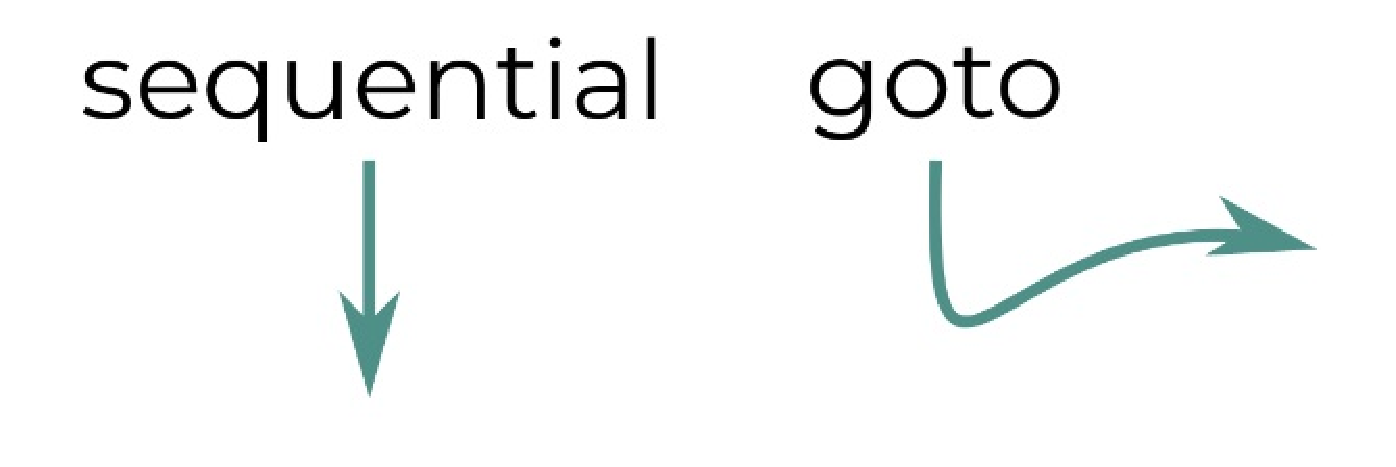
\includegraphics[height=2cm]{./img/goto.eps}
        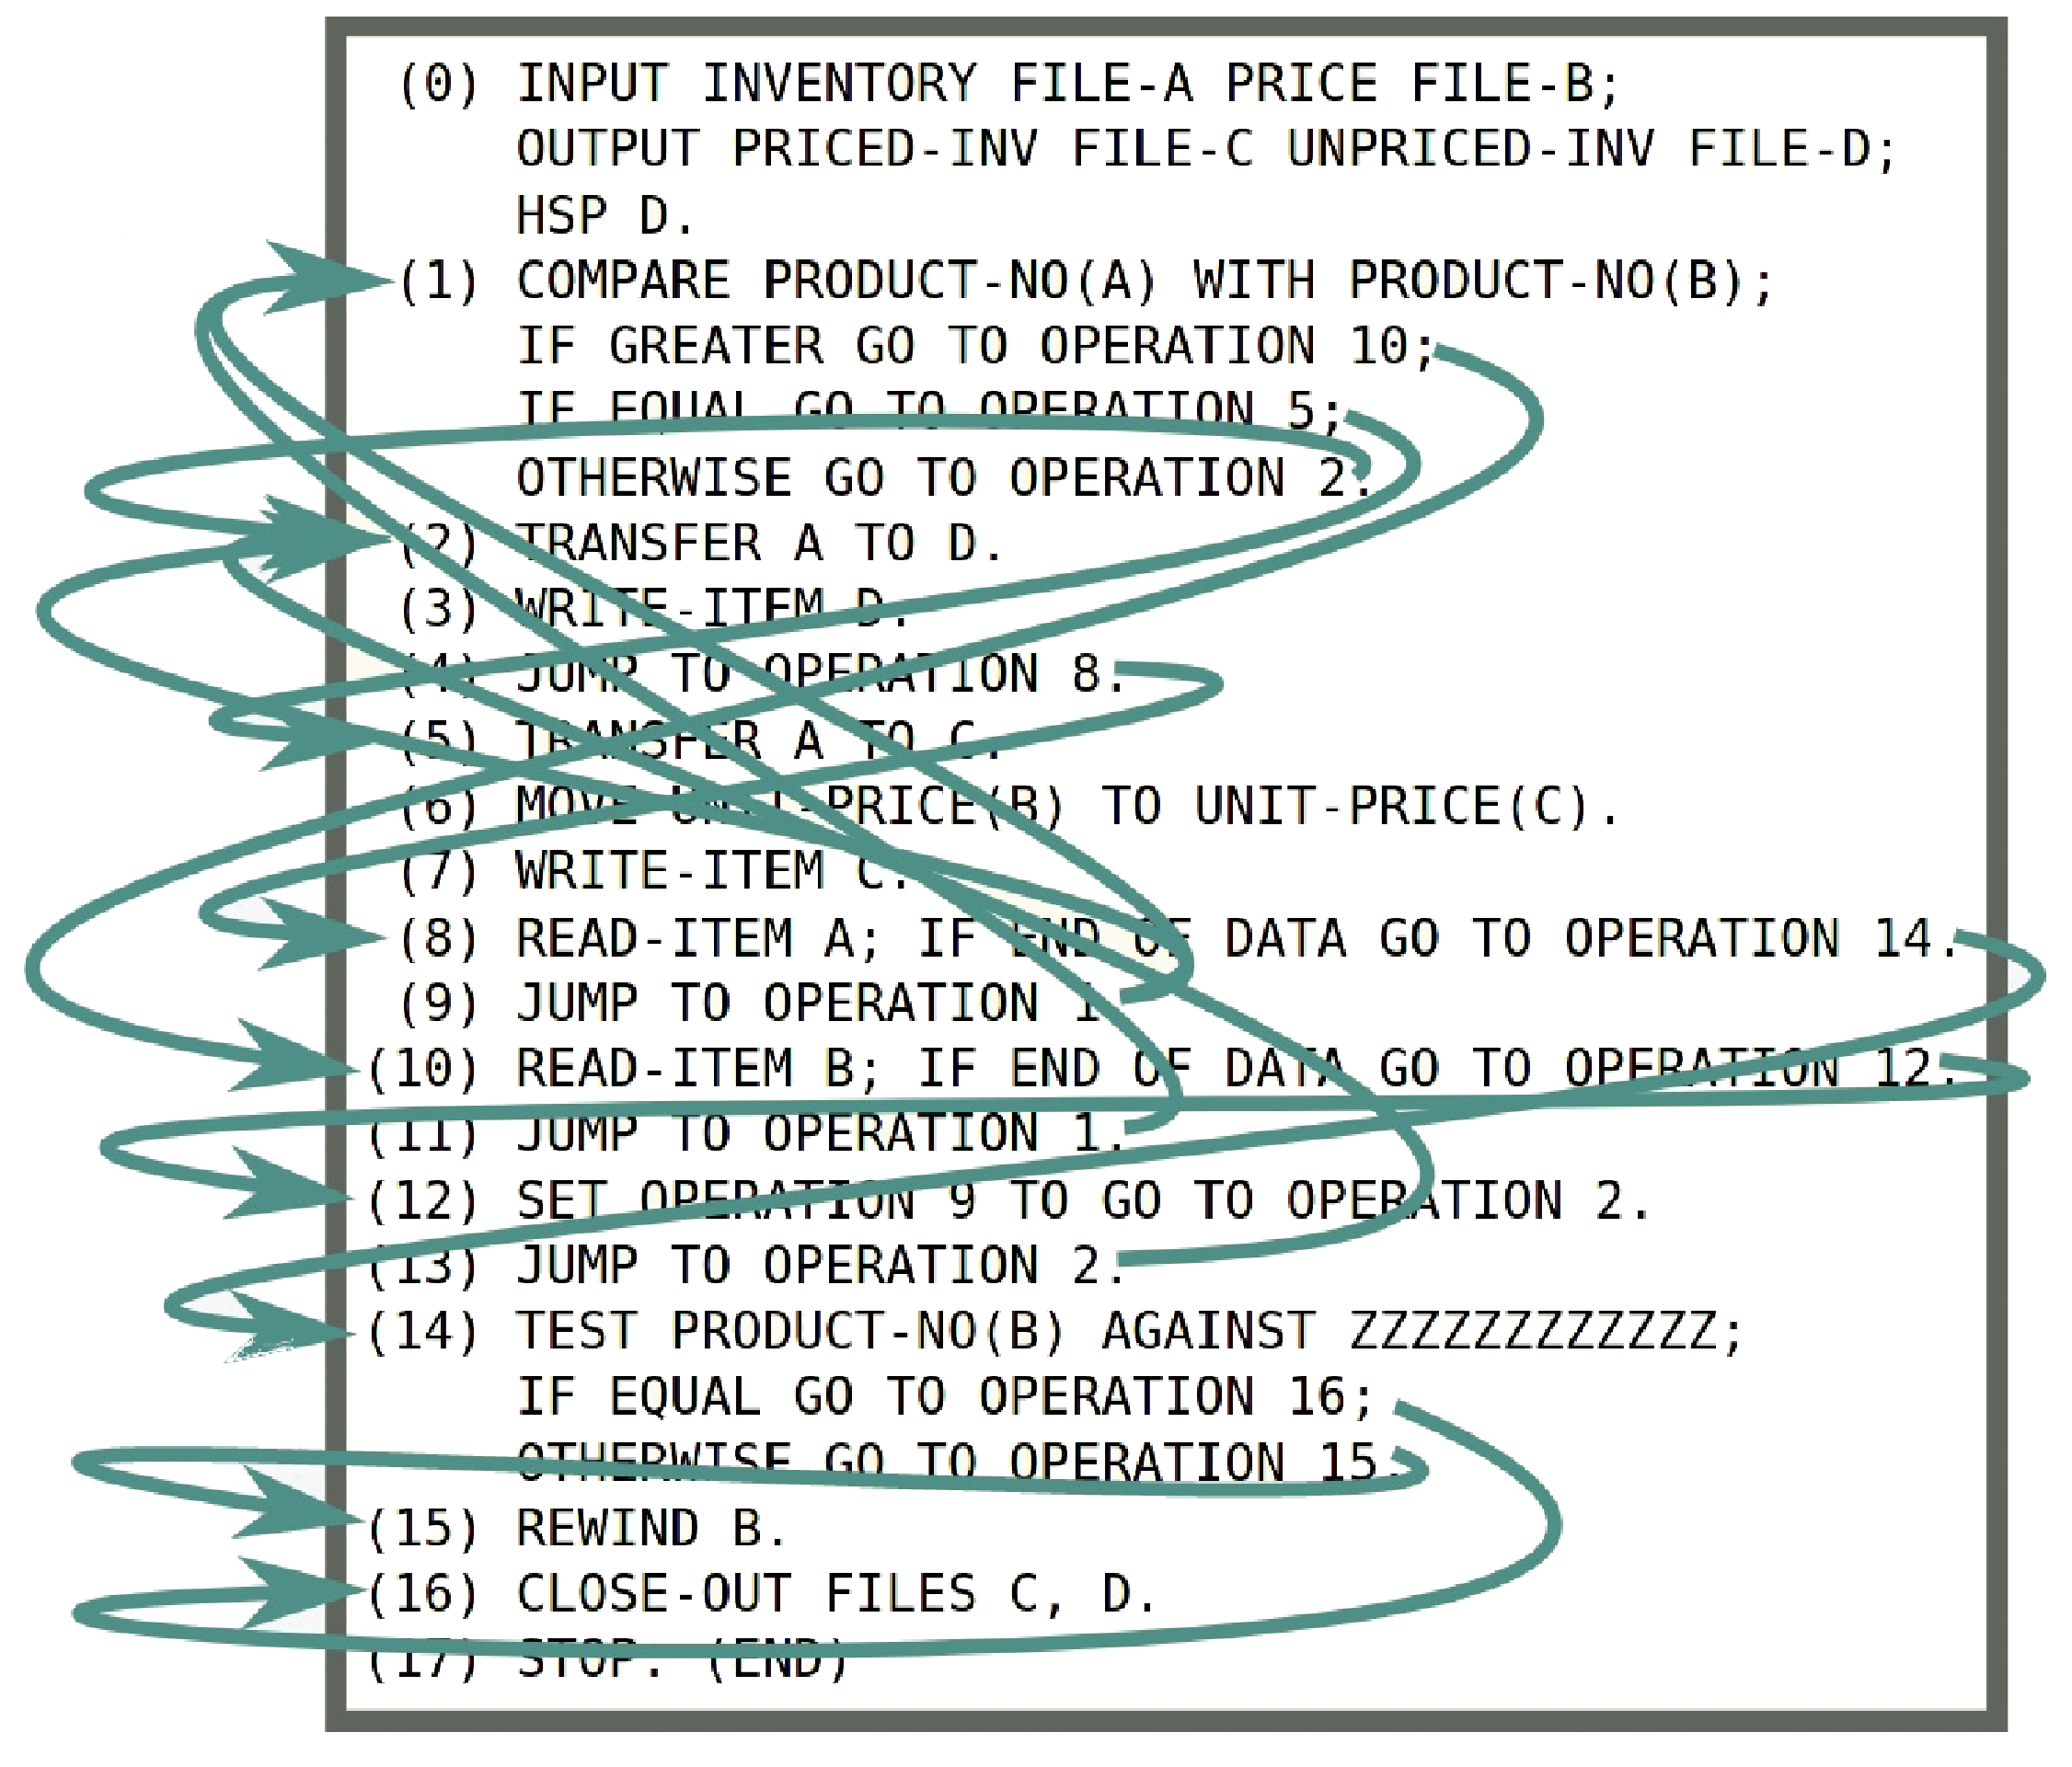
\includegraphics[height=5cm]{./img/goto_example.eps}
        \caption{\tiny{Source: \url{https://vorpus.org/blog/notes-on-structured-concurrency-or-go-statement-considered-harmful/}}}
    \end{figure}
\end{frame}

\begin{frame}
    \frametitle{Structured programming}
    \begin{figure}
        \centering
        Replacing \texttt{goto} with  \texttt{if-else}, \texttt{loop} statements and function calls in 60s:
        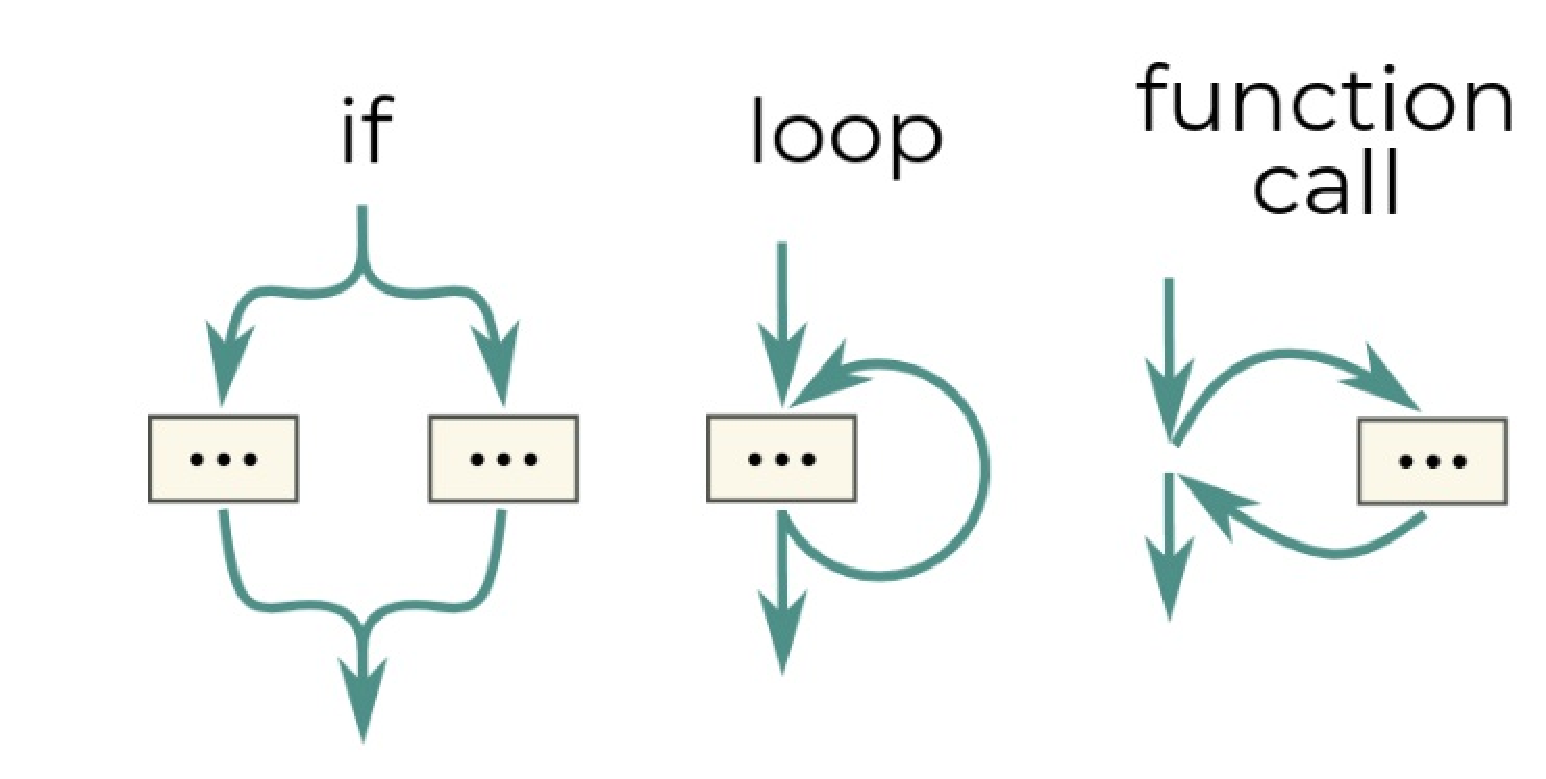
\includegraphics[height=5cm]{./img/structured.eps}
        \caption{\tiny{Source: \url{https://vorpus.org/blog/notes-on-structured-concurrency-or-go-statement-considered-harmful/}}}
    \end{figure}
\end{frame}

\begin{frame}
    \frametitle{Structured concurrency}
    \begin{itemize}
        \item Launching a task in a thread is like using \texttt{goto}.
        \item Structured concurrency is similar to using \texttt{if-else} and \texttt{loop} statements instead of \texttt{goto}.
    \end{itemize}

    \begin{figure}
        \centering
        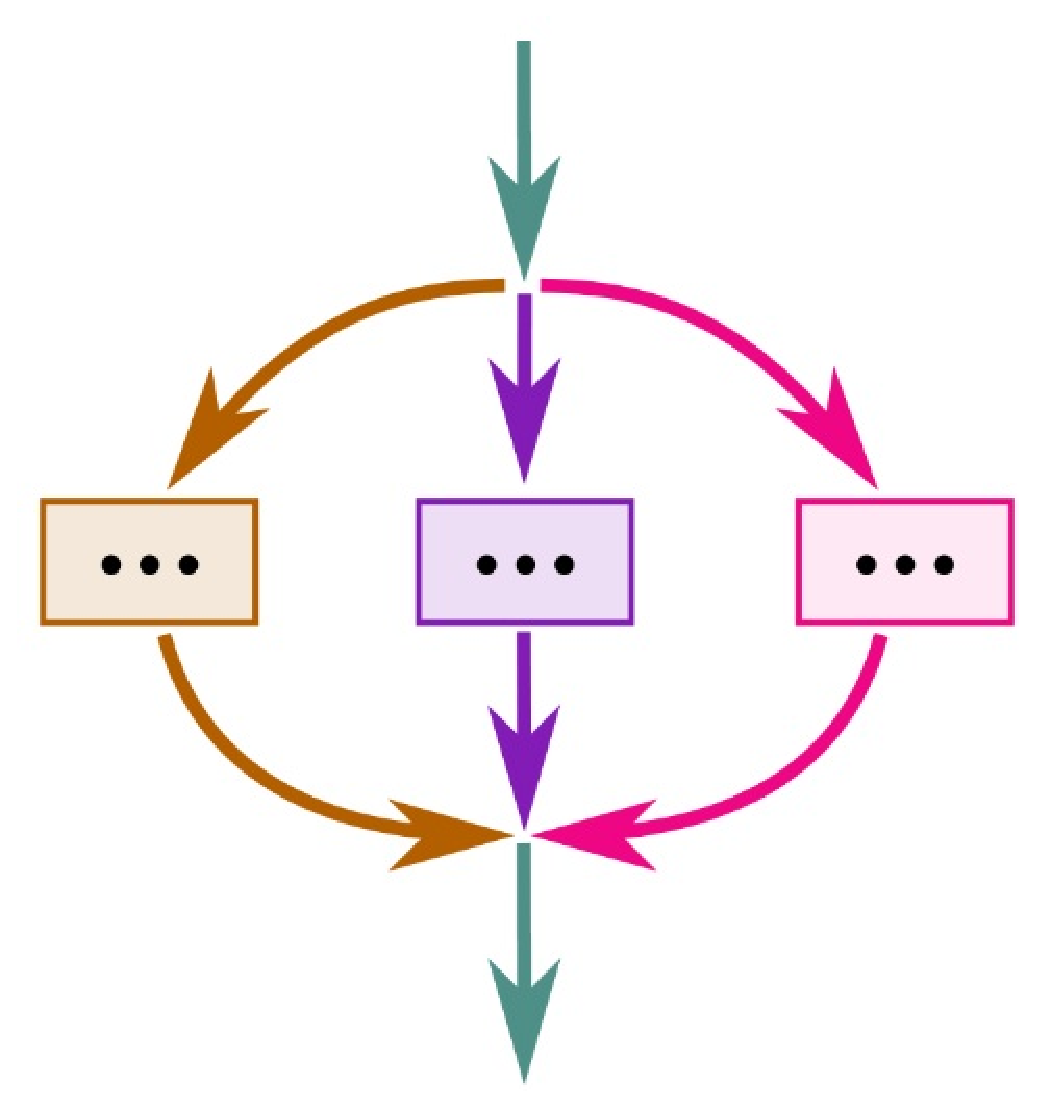
\includegraphics[height=5cm]{./img/structured_concurrency.eps}
        \caption{\tiny{Source: \url{https://vorpus.org/blog/notes-on-structured-concurrency-or-go-statement-considered-harmful/}}}
    \end{figure}
\end{frame}

\begin{frame}[fragile]
    \frametitle{Structured concurrency}

    \begin{lstlisting}[style=java]
try (ExecutorService exec = Executor.newVirtualThreadExecutor()) {
      exec.submit(runable1);
      exec.submit(runable2);
      exec.submit(runable3);
}
    \end{lstlisting}
\end{frame}

\begin{frame}[fragile]
    \frametitle{Structured concurrency: deadlines}

    \begin{lstlisting}[style=java]
ThreadFactory factory = Thread.builder().virtual().factory();
try (var executor = 
    Executors.newThreadExecutor(factory)
    .withDeadline(Instant.now().plusSeconds(30))) {
    executor.submit(task1);
    executor.submit(task2);
}
    \end{lstlisting}
\end{frame}

\begin{frame}
    \frametitle{There is more}
    \begin{itemize}
        \item Structured cancelation.
        \item Scope variables.
        \item Thread local.
        \item $\dots$
    \end{itemize}
    
    \vspace{1cm}
    
    Beware: nothing is set in the store yet, still under development.
\end{frame}

\begin{frame}
    \frametitle{Links}
    \begin{itemize}
    {\scriptsize
        \item \url{http://jdk.java.net/loom/}
        \item \url{https://wiki.openjdk.java.net/display/loom/Main}
        \item \url{https://cr.openjdk.java.net/~rpressler/loom/Loom-Proposal.html}
        \item \url{http://cr.openjdk.java.net/~rpressler/loom/loom/sol1_part1.html}
        \item \url{https://cr.openjdk.java.net/~rpressler/loom/loom/sol1_part2.html}
        \item \url{https://www.javaadvent.com/2020/12/project-loom-and-structured-concurrency.html}
        \item \url{https://blogs.oracle.com/javamagazine/going-inside-javas-project-loom-and-virtual-threads}
        \item \url{https://blog.softwaremill.com/will-project-loom-obliterate-java-futures-fb1a28508232}
        \item \url{https://www.youtube.com/watch?v=fOEPEXTpbJA}
        \item \url{https://www.youtube.com/watch?v=23HjZBOIshY}
        \item \url{https://www.youtube.com/watch?v=_fFzyY_7UmA}
        \item \url{http://belaban.blogspot.com/2020/07/double-your-performance-virtual-threads.html}
    }
    \end{itemize}
\end{frame}

\begin{frame}
    \frametitle{Questions?}
    \centering
     \textbf{\Huge{Thank you!}}
    
    \vspace{1.5cm}
    
    \textbf{\Huge{Questions?}}
    
    \vspace{1cm}
\end{frame}

\end{document}
